\documentclass[first=Christoph,last=Hoentzsch,company=Softwareprojekt,location=Dresden,simple, noheader]{baarticle}

\newacronym{HTTP}{HTTP}{Hypertext Transfer Protocol}
\newacronym{UC}{UC}{Underpinning contract}
\newacronym{ulong}{ulong}{unsigned 64-bit integer}
\addbibresource{simple.bib}
\newglossaryentry{GUI}{
    name=GUI,
    description={Grafische Benutzeroberfläche}
}
\newglossaryentry{UML}{
    name=UML,
    description={Unified Modeling Language}    
}
\newglossaryentry{SCXML}{name=SCXML, description={Statechart-XML}}
\newcommand{\basimpleabstract}{
    \thispagestyle{empty}
    Die vorliegende wissenschaftliche Arbeit wurde mit Unterstützung einer generativen KI erstellt.
    Inhalte wurden teilweise auf Basis der Ausgabe der Künstlichen Intelligenz erstellt, wobei eine eigenständige Überprüfung und wissenschaftliche Validierung durch die Autorin bzw. den Autor erfolgte.
    Die Verantwortung für die Richtigkeit, Vollständigkeit und wissenschaftliche Relevanz der Arbeit liegt bei der Autorin bzw. dem Autor.
    Die Nutzung der KI erfolgte ausschließlich zur Unterstützung der Erstellung und Analyse von Textinhalten im Rahmen der wissenschaftlichen Arbeit.
    Die benutzten Modelle sind GPT 4.1 und GPT 5.
}
\begin{document}
\begin{basimple}[
        img=images/logo.png,
        course=Wirtschaftsinformatik,
        title={Nutzung von Zustandsdiagrammen zur Modellierung von Benutzeroberflächenelementen - eine Fallstudie},
        number=3005551,
        corrector={Prof. Dr. Steffen Greiffenberg},
        themedate={17.12.2025},
        returndate={17.12.2025},
        signature=images/signature.png,
        location=Dresden,
        type=study,
        blocknotice=false,
    ]
    \section{Einleitung} \label{sec:intro}
        Damit Menschen mit Software interagieren können, benötigt es einer Schnittstelle. 
        Um Daten und Informationen an Menschen auszugeben, wird in zeitnaher Software oft eine grafische Benutzeroberfläche (graphical user interface, \gls{GUI}) verwendet.
        Grafische Benutzeroberflächen beanspruchen in der Softwareentwicklung viel Aufmerksamkeit, da sie die Nutzbarkeit von Software stark beeinflussen können.
        Um die Konzeption, Gestaltung und Entwicklung von Benutzeroberflächen zu erleichtern, werden verschiedene Hilfsmittel verwendet. 

        Die Unified Modeling Language (\gls{UML}) ist eine Sprache, mit der Diagramme beschrieben werden können.
        Diese Diagramme können zur Modellierung in der Softwareentwicklung genutzt werden.
        Zustandsdiagramme, StateMachines oder Statecharts können zur Darstellung von endlichen Automaten genutzt werden.
        Sie beschreiben deren Verhalten durch eine Menge an Zuständen und Zustandsübergängen.
        
        In dieser Arbeit soll die Anwendung von \gls{UML} Zustandsdiagrammen in der Entwicklung von grafischen Benutzeroberflächen untersucht werden.
        Dies erfolgt in Form einer Fallstudie.
        Der Anwendungsfall basiert auf der Entwicklung einer Software zur Steuerung einer Gartenbahn mit einem Videospiel-Controller, welche im Rahmen des Moduls \enquote{Softwareprojekt} an der Dualen Hochschule Sachsen in Dresden durchgeführt wurde.

        Das Ziel dieser Arbeit ist es, die folgende Forschungsfrage zu beantworten: 

        \textbf{Wie können \gls{UML}-Zustandsdiagramme in der Entwicklung von Benutzeroberflächen genutzt werden?}

        Um diese Frage zu beantworten, werden im theoretischen Teil dieser Arbeit die Grundlagen zu \gls{UML}-Zustandsdiagrammen, grafischen Benutzeroberflächen und deren Entwicklung erarbeitet. 
        Dabei sollen folgende untergeordnete Forschungsfragen beantwortet werden:

        \begin{itemize}
            \item Wie sind Zustandsdiagramme im Rahmen der \gls{UML} definiert?
            \item Wie werden Zustandsdiagramme angewendet?
            \item Wie werden Benutzeroberflächen entwickelt?
        \end{itemize}

        \newpage
    \section{Theoretischer Hintergrund} \label{sec:theory}
        \subsection{Unified Modeling Language}
        Die Unified Modeling Language (\gls{UML}) ist eine allgemein verwendbare Modellierungssprache.\bacite[22]{Kecher2021}
        Unter Anwendung des semiotischen Dreiecks sind die Diagramme und Diagrammelemente die Zeichen, das Modell der Begriff und der modellierte Gegenstand das Objekt.
        Ein Modell stellt eine Abstraktion des modellierten Gegenstandes dar, wobei bei \gls{UML} Modellen zusätzlich die Perspektive und das Ziel des Modells betrachtet werden.\vglcite[12]{OMG2017}\vglcite[9]{Rumpe2011}
        Als Zweck der Modellierung wird in einigen Begriffsdefinitionen die Erleichterung einer Untersuchung gegeben.\vglcite[9]{Rumpe2011}
        Der modellierte Gegenstand sind in der \gls{UML} im allgemeinen Systeme, welche durch Klassifikatoren bezeichnete Objekte, Ereignisse und Verhalten enthalten.\vglcite[12]{OMG2017}
        Die \gls{UML} kann in verschiedensten Anwendungsgebieten angewendet werden.\vglcite[22]{Kecher2021}
        Der Hauptanwendungsbereich ist die Softwareentwicklung.\vglcite[22]{Kecher2021}\vglcite[1]{OMG2017}

        Die \gls{UML} unterscheidet die \gls{UML} Diagrammelemente in verschiedene zwei verschiedene semantische Gebiete, die sich über die zeitliche Betrachtung unterscheiden.
        Strukturelemente für Objekte werden durch die Struktursemantik definiert und können zu einem bestimmten Zeitpunkt wahr sein.
        Verhaltenselemente werden durch die Verhaltenssemantik definiert und beschreiben Objekte über einen bestimmten Zeitraum.\vglcite[13]{OMG2017}
        Daraus entstehen drei Modellierungsarten:\vglcite[14]{OMG2017}\vglcite[26]{Kecher2021}
        \begin{itemize}
            \item Strukturmodellierung (enthält Elemente für Klassifikatoren, Pakete, Werte, Klassen, etc.)
            \item Verhaltensmodellierung (enthält Elemente für Zustandsmaschinen, Aktivitäten, Interaktionen, Aktionen, etc.)
            \item Ergänzungsmodellierung (enthält Elemente für Anwendungsfälle, Deployments, Informationsflüsse)
        \end{itemize}
        Die Abbildung \ref{fig:diagramtypes} stellt eine Übersicht über die Diagrammarten, die mit der \gls{UML} assoziiert werden, da.

        \begin{bafigure}[
            source={\captioncite{Kecher2021}},
            label={fig:diagramtypes}
        ]{Diagrammarten der \gls{UML}}
            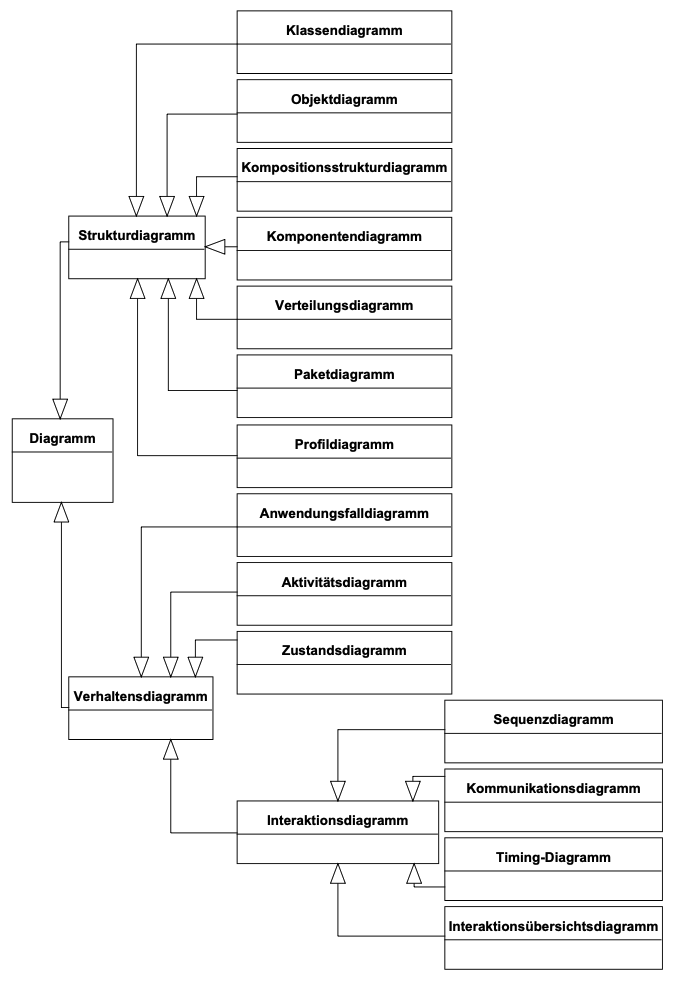
\includegraphics[width=14cm]{images/Diagrammarten.png}
        \end{bafigure}

        \newpage

        \subsection{Zustandsdiagramme}
            \subsubsection{Definition}

            Zustandsdiagramme sind Teil der Verhaltensmodellierung.
            Sie basieren auf dem \enquote{Statechart} Formalismus von David Harel.\vglcite[305]{OMG2017}\vglcite{Harel1986}
            Zustandsdiagramme modellieren das diskrete ereignis-basierte Verhalten des modellierten Gegenstandes in Form von endlichen Zustandsautomaten. \vglcite[305]{OMG2017}
            Es wird in zwei verschiedene Arten von Zustandsdiagrammen unterschieden: \enquote{Verhaltenszustandsdiagramme} (behavior state machines) stellen das Verhalten eines Objekts dar, während \enquote{Protokollzustandsdiagramme} (protocol state machines) die möglichen Interaktionssequenzen für Objekte darstellen. \vglcite[305]{OMG2017}
            In dieser Arbeit werden nur Verhaltenszustandsdiagramme betrachtet, da diese im praktischen Fall angewendet wurden. 
            Die folgende Beschreibung von (Verhaltens-) Zustandsautomaten wurde aus der \gls{UML} Spezifikation Sektion 14.2.3 und aus Rumpe 2011 Kapitel 5.3f entnommen.\vglcite[306-318]{OMG2017}\vglcite[150ff]{Rumpe2011}.

            Ein Zustandsautomat ist zusammengesetzt aus Regionen, die einen Graph aus Eckpunkten und Kanten enthalten.
            Die Eckpunkte des Graphen können Zustände, Pseudozustände oder Verbindungspunkte darstellen.
            Die Kanten des Graphen stellen Transitionen dar.

            Ein Zustand ist eine Situation während der Ausführung des Zustandsautomaten, in der eine bestimmte Bedingung gilt.
            Diese Bedingung wird meist durch den Namen des Zustands impliziert.
            Ein Zustand kann verschiedene interne Verhalten/Aktionen besitzen, die bei dem Betreten (entry), nach dem Betreten für die Dauer des Zustands (do) und nach dem Verlassen des Zustands (exit) ausgeführt werden.
            Es existieren drei Arten von Zuständen:
            \begin{itemize}
                \item Simple Zustände enthalten keine Graphen
                \item Zusammengesetzte Zustände enthält mindestens eine Region
                \item Unterzustandsautomatenzustände enthalten einen Zustandsautomat
            \end{itemize}
            Zusammengesetzte Zustände können zudem eine Historie besitzen, welche die Zustandskonfiguration vor dem letzten Verlassen des Zustands darstellen.
            Die Tiefhistorie und die Flachhistorie unterscheiden sich in der Tiefe der \enquote{gemerkten} Zustände; die Tiefhistorie merkt sich die vollständige Zustandskonfiguration, während sich die Flachhistorie nur die oberste Teilzustandsebene merkt.
            Der sog. Endzustand zeigt an, dass die Ausführung einer Region vollendet ist.

            Pseudozustände sind sehr kurzweilige Situationen, die während der Ausführung des Zustandsautomaten angenommen werden können.
            Relevant ist für diese Arbeit der Startzustand, der den Startpunkt für eine Region darstellt und von dem die Region bei Standardeintritt ausgeführt wird.
            Verbindungspunkte können Ein- und Austrittspunkte für Unterzustandsautomatenzustände darstellen.

            Transitionen sind gerichtete Übergänge zwischen einem Quelleckpunkt und eine Zieleckpunkt und stellen einen Teil des Verhaltens des Zustandsautomaten dar. 
            Eine Transition wird ausgeführt, wenn ein Event für einen Stimulus (trigger) der Transition eintritt und wenn sich der Zustandsautomat an der Quellkante befindet.

            Zustandsdiagramme stellen Zustandsautomaten grafisch dar. Die voran beschrieben Elemente sind in Abbildung \ref{fig:diagramelements} in der \gls{UML} Notation dargestellt.

            \begin{bafigure}[
                source={Eigene Darstellung},
                label={fig:diagramelements}
            ]{Elemente von Zustandsdiagrammen}
                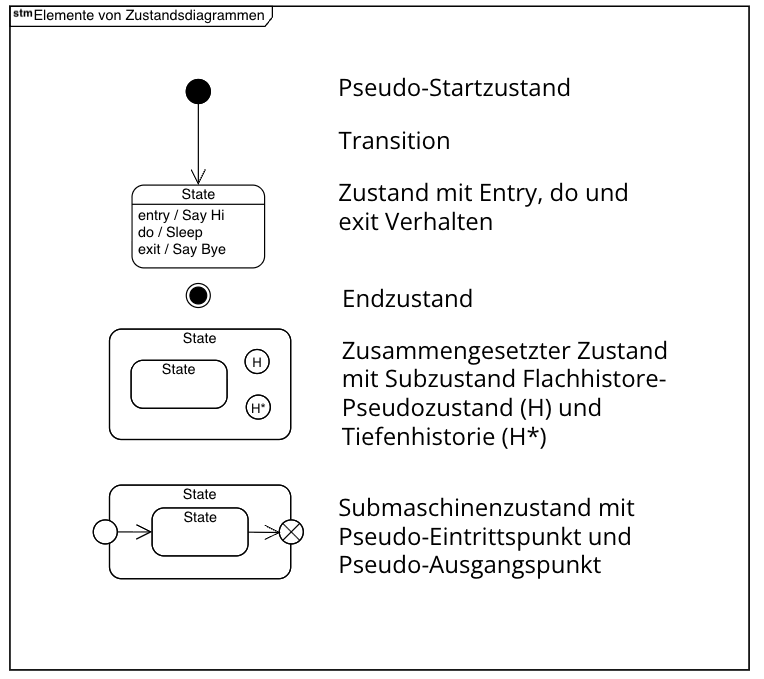
\includegraphics[width=14cm]{images/Statemachineelements.png}
            \end{bafigure}

            \subsubsection{Anwendung}
            Die Zustandsautomaten und die vorausgehenden Statecharts basieren auf der finiten Automatentheorie.
            Es kann dabei in zwei Typen von Automaten unterschieden werden:\bacite[151-152]{Rumpe2011}
            \begin{itemize}
                \item Erkennende Automaten durchlaufen für ein Eingabealphabet eine Menge an Zuständen durch Transitionen von einem Start- zu einem Endzustand. Eine Definition ist in Abbildung \ref{fig:automat1} zu finden.
                \item Mealy-Automaten geben zusätzlich an jeder Transition ein Element eines Ausgabealphabets aus. Eine Definition ist in Abbildung \ref{fig:automat2} zu finden.
            \end{itemize}

           
            \begin{bafigure}[
                source={\captioncite{Rumpe2011}},
                label={fig:automat1}
            ]{Definition Finiter Zustandsautomat}
                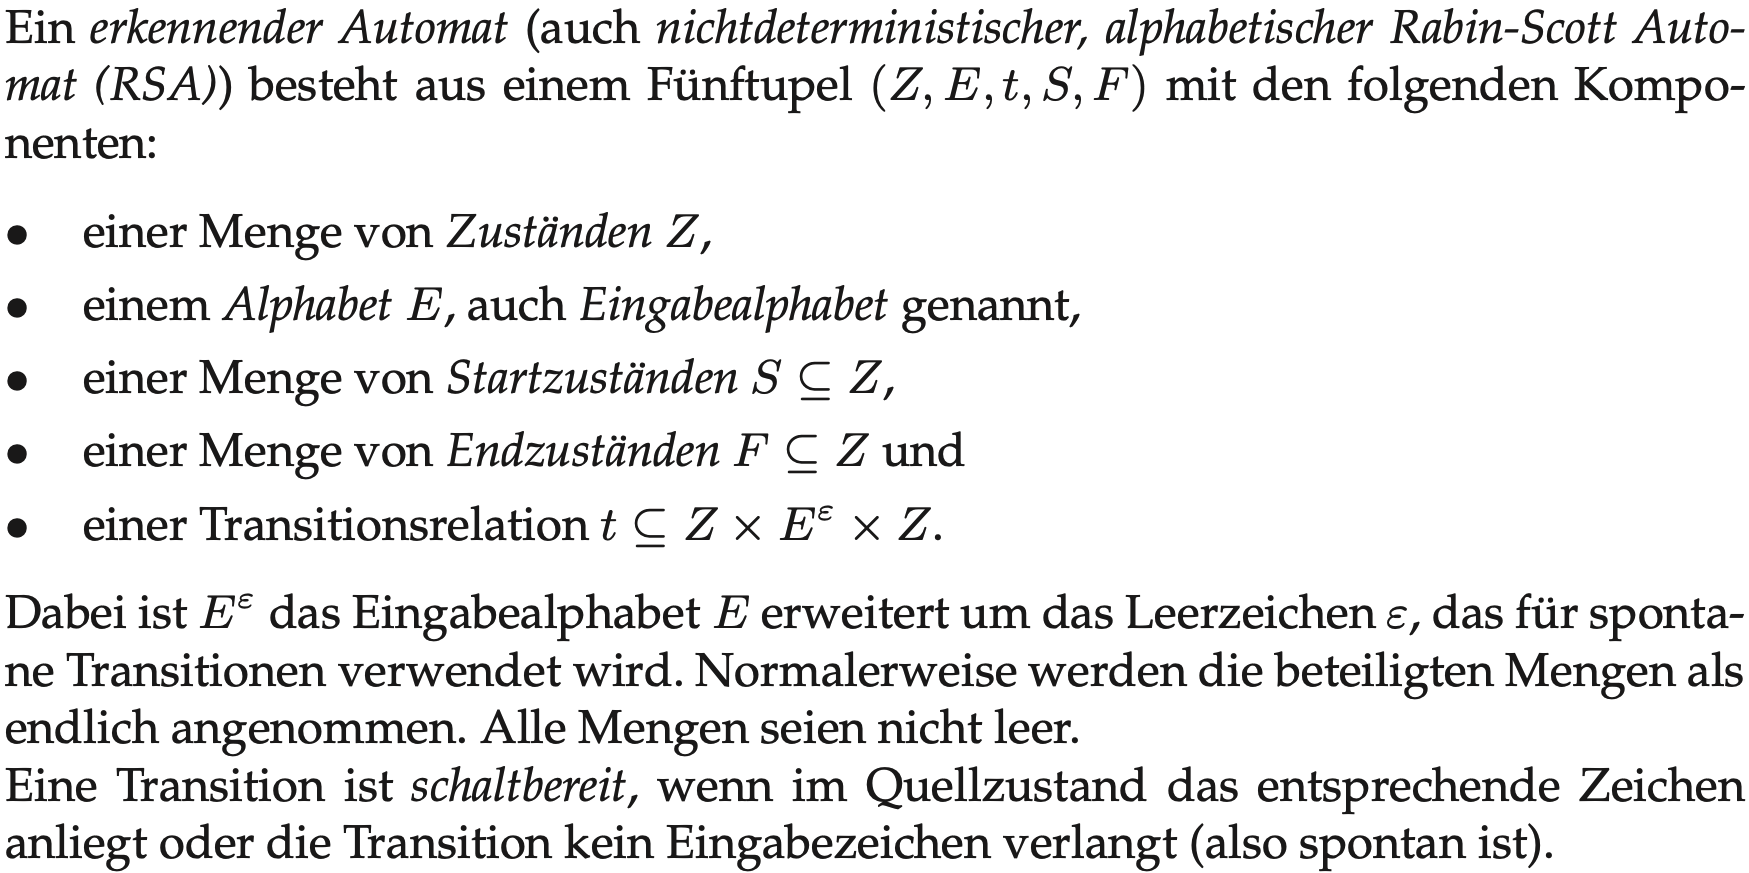
\includegraphics[width=14cm]{images/Automat.png}
            \end{bafigure}
            \begin{bafigure}[
                source={\captioncite{Rumpe2011}},
                label={fig:automat2}
            ]{Definition Mealy-Automat}
                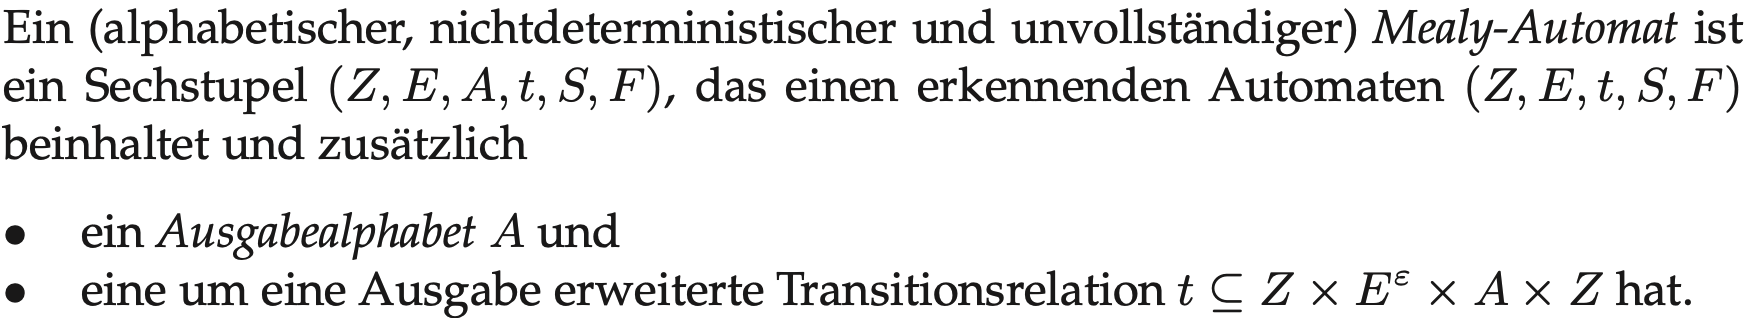
\includegraphics[width=14cm]{images/Mealy.png}
            \end{bafigure}

            Aufgrund des hohen Grades an Abstraktion der Automatentheorie kann sie auf zahlreiche Gebiete angewendet werden.
            Die von Rumpe formulierten Aufgaben Aufgaben, die ein Zustandsdiagramm in der Objektorientierten Softwareentwicklung übernehmen kann, werden in Abbildung \ref{fig:usecases} dargestellt:\bacite[149]{Rumpe2011}

            \begin{bafigure}[
                source={\captioncite{Rumpe2011}},
                label={fig:usecases}
            ]{Aufgaben eines Statecharts}
                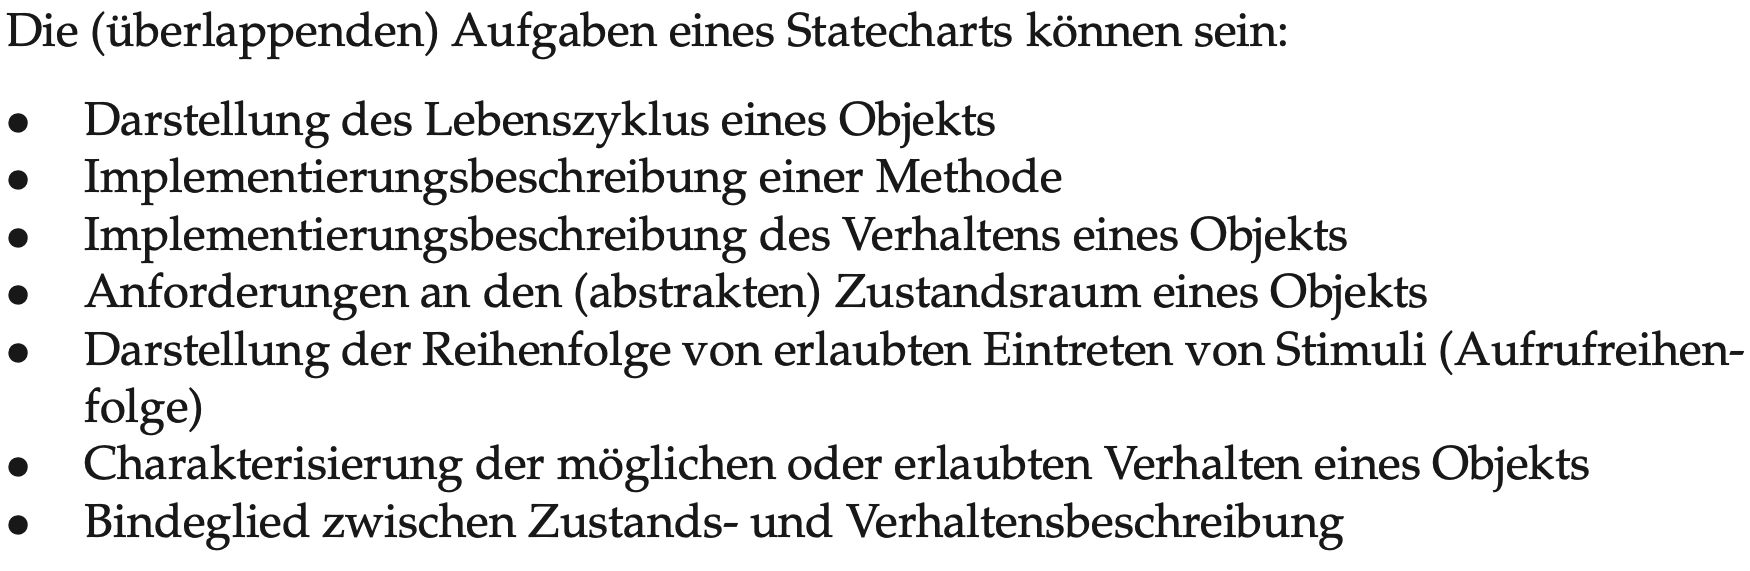
\includegraphics[width=14cm]{images/AufgabenStatechart.png}
            \end{bafigure}

            In konkreten Anwendungsszenarien können Zustandsdiagramme unter anderem für Softwaretesting und die Erstellung von Testfällen \vglcite{Aggarwal2012}\vglcite{Felderer2014}, zur Automation in der Fertigung \vglcite{Guo2007} oder für Automatische Code Generierung \vglcite{Samuel2019} genutzt werden.
            
            \newpage
        \subsection{Grafische Benutzeroberflächen}
            \subsubsection{Definition}
            Eine grafische Benutzeroberfläche (auch Benutzeroberfläche, GUI oder UI) ist eine Schnittstelle zwischen Menschen und Maschinen.\vglcite[4]{Chlebek2011}\vglcite[1]{Jansen1998}\vglcite[1]{Martinez2011}\vglcite[150]{Heinzl2024}
            Der Mensch benutzt die Benutzeroberfläche, um der Maschine Anweisungen zu geben und Informationen aufzunehmen.\vglcite[1]{Jansen1998}\vglcite[1]{Martinez2011}
            Benutzeroberflächen sind meist Ereignis-basiert; eine Aufgabe wird im Programm ausgeführt, wenn der Nutzer eine Aktion ausführt, beispielsweise das \enquote{klicken} eines Elements der grafischen Benutzeroberfläche.\vglcite[1]{Martinez2011}
            Die Benutzeroberfläche kann dabei effektiv einschränken, welche Aufgaben ausgeführt werden können.\vglcite[1]{Jansen1998}
            Grafische Benutzeroberflächen enthalten und nutzen in ihrer Darstellung meist Fenster, Symbole, Menüs, Knöpfe, Dropdowns, Eingabefelder und Zeiger.\vglcite[1]{Martinez2011}\vglcite[1]{Jansen1998}
            Grafische Benutzeroberflächen werden oft mit der Befehlszeile in Kontrast gesetzt, welche dem Nutzer keinen Kontext geben und Vorkenntnisse über das laufende Programm voraussetzen.\vglcite[1]{Martinez2011}\vglcite[1]{Jansen1998}

            \subsubsection{Entwicklungsprozess}
            Der Entwicklungsprozess von grafischen Benutzeroberflächen und der allgemeine Entwicklungsprozess sind stark miteinander verknüpft.\vglcite[318]{Lukin2019}
            Allgemein gilt, dass die Phasen, die allgemein bei der Softwareentwicklung durchlaufen werden, ebenfalls bei der Entwicklung von grafischen Benutzeroberflächen auftreten, da letzteres Teil des ersteren ist.
            Modelle wie das Wasserfallmodell oder das Inkrementelle Entwicklungsmodell mit Methoden wie Scrum oder Test-Driven Development können auch den Rahmen für die Entwicklung von grafischen Benutzeroberflächen bilden.\vglcite[47-50]{Sommerville2016}
            %Hier noch Abbildungen der Modelle
            
            Besonders anzumerken ist, dass die Nutzerzentrierung bei der Benutzeroberflächenentwicklung stark betont wird, weil Endnutzer auf die Nutzbarkeit der Benutzeroberfläche angewiesen sind.\vglcite[317f]{Lukin2019}\vglcite[29ff]{Chlebek2011}
            In der Analyse und im Entwurf sind Techniken wie Anwendermodelle, Anforderungsinterviews oder Storyboards explizit auf die nutzerzentrierte Anforderungserhebung ausgelegt.\vglcite[44]{Chlebek2011}
            Die Nutzung von Dialogseitendiagrammen und Screendesigns kann Entwicklern in der Entwurfsphase helfen bei der Veranschaulichung und können iterativ eingesetzt werden, um Nutzerfeedback zu sammeln.\vglcite[66f]{Chlebek2011}
            Die Erstellung von Prototypen in der Benutzeroberflächenentwicklung dient nicht nur der Verifizierung, sondern mithilfe von Nutzertests auch der Validierung.\vglcite[129ff]{Chlebek2011}\vglcite[62ff]{Sommerville2016}
            Außerdem werden in der Entwicklung von Benutzeroberflächen dem (initialen) Design und dem Redesign (Verbesserung von etwas Bestehendem aufgrund von Nutzerfeedback) ähnliche Priorität gegeben.\vglcite[161ff]{Chlebek2011}

            Für die Programmierung von grafischen Benutzeroberflächen existieren je nach Plattform eine hohe Anzahl an verschiedenen Werkzeugen, Bibliotheken und Frameworks.
            Für die Android Plattform ist Jetpack Compose eine offiziell (von Google, Inhaber von Android) unterstützte UI-Bibliothek.
            Jetpack Compose baut deklarativ grafische Benutzeroberflächen.
            Elemente der Benutzeroberfläche werden als im Code als Funktionen dargestellt, welche wiederverwendet und ineinander verschachtelt werden können.
            Daten aus der Geschäftslogik können dabei als Parameter an die Elemente weitergegeben werden.
            Die lokale Compose-Laufzeit übernimmt die Komposition (initialer Aufbau der Benutzeroberfläche) und Rekomposition (Aktualisierung der Elemente basierend auf Ereignissen/Datenänderungen). 
            Jetpack Compose nutzt zudem Kotlin, was die Einbindung in Android stark erleichtert.\vglcite[2-8]{Asefa2022}

            \newpage
        \subsection{Zustandsdiagramme in der Entwicklung von grafischen Benutzeroberflächen}
        Wie in sonstigen Softwareentwicklung können auch in der Entwicklung von Benutzeroberflächen \gls{UML}-Diagramme zum Zweck der Modellierung eingesetzt werden. 
        Chlebek nennt unter anderem Klassendiagramme, Use-Case-Diagramme und Robustheitsdiagramme als Analyse- und Entwurfswerkzeuge. \vglcite[44]{Chlebek2011}
        In einem Nebensatz wird die Nutzung von Statecharts zur Modellierung von Interaktionen erwähnt (wobei Rumpe\vglcite[149]{Rumpe2011} widersprechen würde, laut ihm sollten Zustandsdiagramme nur zur Modellierung Objektverhalten genutzt werden).
        
        Kistner und Nuernberger von NVIDIA\vglcite{Kistner2014} haben die Anwendung \enquote{Architect} entwickelt.
        Die Anwendung basiert auf \enquote{NVIDIA's UI Composer Studio}, einer Anwendung zur Erstellung von 3D-Benutzeroberflächen.
        Das Ziel der Anwendung war, visuelle Zustandsänderungen von ihren Auslösern, um den Entwicklungsprozess zu erleichtern.
        Für die Darstellung der logischen Zustände wurden Zustandsdiagramme genutzt.
        \enquote{Architect} ist ein visueller Editor und erlaubt die Erstellung und Modifizierung von \gls{SCXML} (Statechart-XML) Dateien.
        Mit Hilfe einer zwischengestellten Runtime wurde die Zustandssteuerung von Benutzeroberflächen mit \gls{SCXML}-Zustandsdiagrammen realisiert.

        Besonders relevant ist hier die Arbeit von Nguyen.\vglcite{Nguyen2020}
        In deren Arbeit werden Zustandsdiagramme genutzt um das Verhalten der Musikspielapplikation \enquote{XTune} zu modellieren.
        Für die Programmierung der App wurde Vuex, ein progressives Webframework, genutzt, das in seiner Funktionsweise Jetpack Compose ähnelt.
        Zuerst wurden Funktionen der Anwendung als funktionale Anforderungen in Form von User-Stories definiert.
        Anschließend wurden für die einzelnen Funktionen jeweils ein Zustandsdiagramm modelliert.
        Die Modelle wurden auf Validität, Erreichbarkeit der Zustände, Determinismus und sog. \enquote{Deadlock}-Zustände (Zustände, die nicht terminieren und nicht gewollt sind) geprüft.
        Mit Hilfe von XState, einem Typescript-basierten \gls{SCXML}-Interpreten, wurden die Zustandsdiagramme in der Applikation umgesetzt.

        \newpage
    \section{Methodik} \label{sec:meth}   
        \subsection{Forschungsmethode}
        Diese Arbeit ist die Prüfungsleistung im Modul \enquote{Softwareprojekt} an der Dualen Hochschule Sachsen in Dresden.
        Die Auswahl der Fallstudie als Forschungsmethode liegt in der Vorgabe durch den Dozenten begründet.

        Fallstudien ordnen sich in die empirische qualitative Forschung ein.\vglcite[113]{Ridder2020}
        Das Subjekt der Fallstudie ist ein aktuelles, soziales Phänomen mit seinem Kontext in der realen Welt; der Fall.\vglcite[113]{Ridder2020}\vglcite[117]{Riedel2006}
        Jene Fälle können unter anderem Individuen, kleine Gruppen, Organisationen, Projekte, Gemeinschaften, Beziehungen, Entscheidungen oder Partnerschaften sein.\bacite[71]{Yin2018}
        Die Daten können aus verschiedenen Quellen wie Dokumenten, Interviews, Observation(sprotokolle) oder physischen Artefakten erhoben werden.\vglcite[86]{Ridder2020}\vglcite[65]{Heinzl2024}
        Fallstudien können anhand der Anzahl von betrachteten Fällen in Einzelfallstudien (ein Fall) und vergleichende Fallstudien (mehrere Fälle) unterschieden werden.\vglcite[117ff]{Ridder2020}
        Riedl unterscheidet zudem auf Basis des Zwecks in Deskriptive Fallstudien (Beschreibung von Artefakten, Sachverhalten, Ereignissen und Handlungen), Explorative Fallstudien (Generierung von Hypothesen) und Explanative Fallstudien (Testung von Theorien).\vglcite[130f]{Riedel2006}

        \subsection{Vorgehen}
        Diese Fallstudie ist als deskriptive Fallstudie konzipiert. 
        Zudem wird in dieser Fallstudie ein Einzelfall betrachtet.
        Beide Entscheidungen werden durch den limitierten zeitlichen Rahmen begründet.
        
        In dem folgenden Kapitel erfolgt eine Beschreibung des Falls.
        Anschließend sollen Daten aus dem Fall analysiert werden.
        Als Datenquellen sollen folgende Dokumente und digitale Artefakte betrachtet werden.
        \begin{itemize}
            \item Zustandsdiagramme
            \item Software Requirements Specification
            \item Quellcode der Software
            \item Bildschirmfotos der Benutzeroberfläche
        \end{itemize}
        In der Datenanalyse soll der Zweck der Nutzung der Zustandsdiagramme identifiziert werden.
        Mithilfe der Software Requirements Specification, dem Quellcode der Software und den in Kapitel \ref{sec:theory} beschriebenen theoretischen Grundlagen sollen die Zustandsdiagramme validiert und verifiziert werden.
        Der Zweck der Datenanalyse ist die Beantwortung der in Kapitel \ref{sec:intro} gestellten Forschungsfrage.

        Es ist zu erwähnen, das der Autor dieser Arbeit in dem Fall umfänglich als Akteur beteiligt war.
        Trotzdem soll in dieser Arbeit ein neutral beobachtender Standpunkt angenommen werden.

    \newpage
    \section{Empirische Beobachtung} \label{sec:case}
    \subsection{Fallbeschreibung}
        \subsubsection{Das Gartenbahnprojekt}
        Das Modul \enquote{Softwareprojekt} an der Dualen Hochschule Sachsen in Dresden wird anhand einer \enquote{Gartenbahn} durchgeführt. 
        Die Gartenbahn konstituiert mehrere hölzerne Kästen, auf denen unter anderem Miniaturmodelle von Kränen, Bahnhöfen und Landschaftselementen, und stromleitende Miniaturschienen der Spurweite G angebracht sind. 
        Jene stromleitende Schienen können Miniaturlokomotiven antreiben.
        Die Lokomotiven und diverse andere Miniaturmodelle der Gartenbahn (Weichen, Kräne, Schranken) sind mit Raspberry Pi's ausgestattet (Modellserver), welche eine kabellose Steuerung der ermöglichen. 
        An der Unterseite der Module sind ebenfalls Raspberry Pi's angebracht, die als Namensserver für die Modellserver fungieren.

        Wenn die Gartenbahn an Strom angeschlossen wird, versuchen sich die einzelnen Modellserver mittels HTTP-Anfragen bei einem Namensserver \enquote{anzumelden}. 
        Ist die Anmeldung erfolgreich, können die jeweiligen Modellserver mittels einer HTTP-GET-Anfrage an den Namensserver ermittelt werden. 
        Um die einzelnen Modellserver anzusprechen, wurde von dem Dozenten der Vorlesung ein Client für Android-Geräte in Kotlin entwickelt.
        Der Client führt die oben beschriebene HTTP-Get-Anfrage durch und zeigt die zurückgegebenen Server als Elemente der Gartenbahn an. 
        Wird ein bestimmtes Modell ausgewählt, baut der Client eine Websocket-Verbindung mit dem korrespondierenden Modellserver auf.
        Der Client stellt die verschiedenen Attribute des Modellobjekts mittels seiner grafischen Benutzeroberfläche dar.
        Die Benutzeroberfläche des Clients ist in Abbildung \ref{fig:oldUI} dargestellt.
        Über die Benutzeroberfläche können die Attribute des Modells wie beispielsweise die Geschwindigkeit einer Lokomotive geändert werden.
        Durch dieses Prinzip können die Elemente der Gartenbahn gesteuert werden.
        \begin{bafigure}[
                source={Eigene Darstellung},
                label={fig:oldUI}
            ]{Benutzeroberfläche des Clients. Die obere Tableiste stellt die Liste an verfügbaren Modellen dar}
                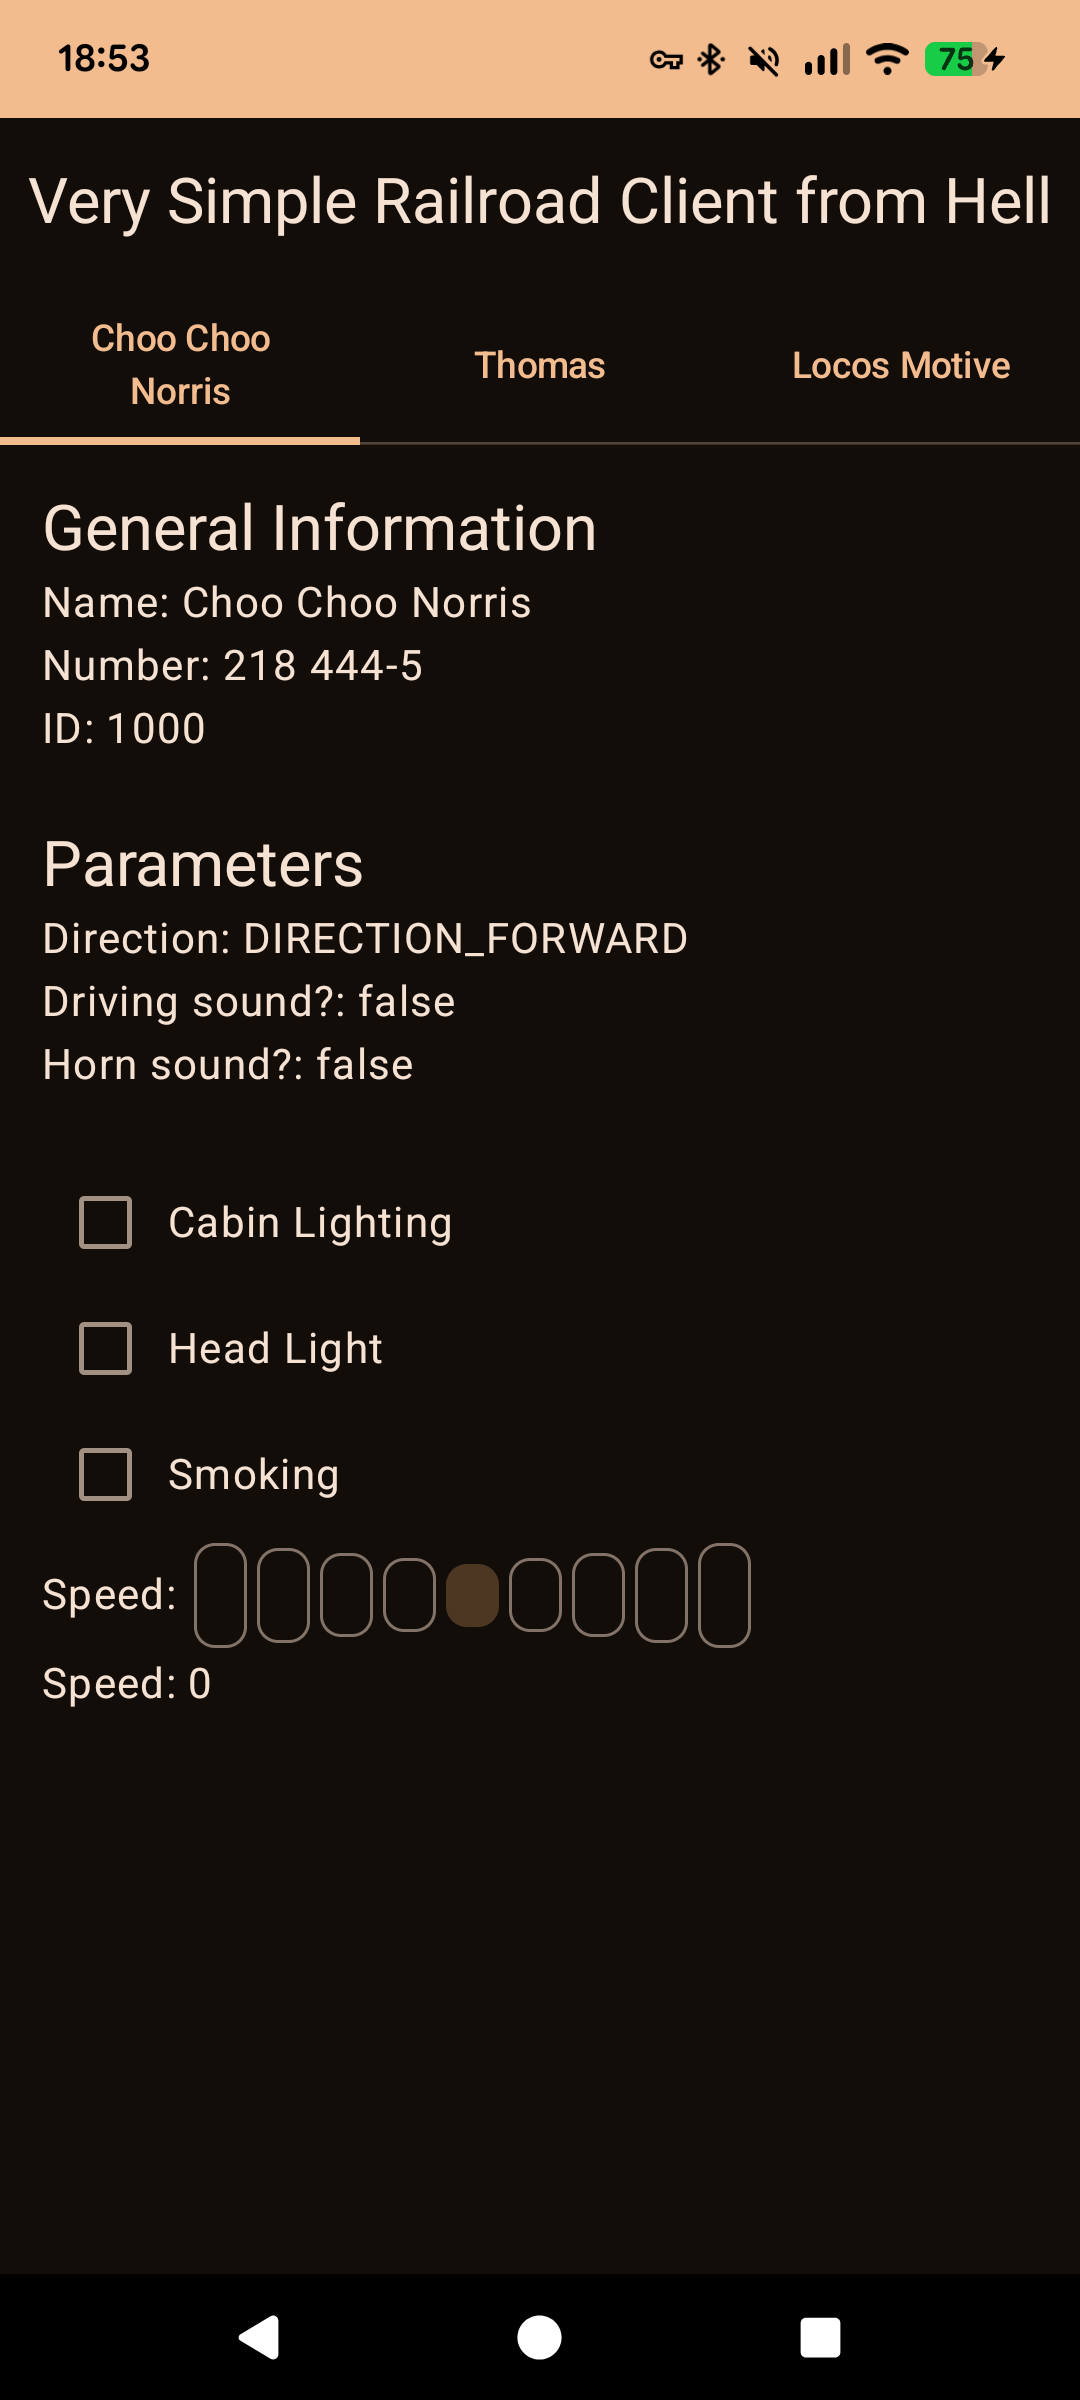
\includegraphics[width=4cm]{images/UIold.png}
        \end{bafigure}

        \subsubsection{Der Controlleur}
        Im Rahmen des Softwareprojekts entschied sich die Gruppe 2 mit den Mitgliedern Jessica Driver, Pia Ihbe, Miriam Herzog, Benjamin Lehmann, Luca Schubert und Christoph Höntzsch für die Entwicklung einer Viedospielcontrollersteuerung der Gartenbahn, spezifisch die Steuerung von Lokomotiven/Bahnen. 
        Das resultierende Produkt trägt den Namen \enquote{Der Controlleur} und wurde von dem fiktiven Unternehmen \enquote{ControlWare} entwickelt.

        Die Anforderungserhebung wurde durch eine Online-Umfrage durchgeführt, welche durch die Teammitglieder Benjamin Lehmann, Miriam Herzog und Jessica Driver konzipiert wurde. Anhand der Ergebnisse wurde eine Persona erstellt und Anforderungen wurden in die Software Requirements Specification übernommen. 
        Im Anschluss wurde die Softwarearchitektur durch Pia Ihbe festgelegt.
        Aus zeitlichen und Komplexitätsgründen wurde entschieden, die bestehende Client App mit der Controllersteuerung zu erweitern.
        Die Entwicklung der funktionalen Einbindung des Controllers fand durch Luca Schubert statt.
        Für ein Redesign der Benutzeroberfläche war Christoph Höntzsch verantwortlich.
        Für die Entwicklung der Benutzeroberfläche wurde GitHub Copilot mit GPT4.1 als Basismodell unterstützend genutzt.

        \subsubsection{Redesign der Benutzeroberfläche}
        Aufgrund des limitierten zeitlichen Rahmens wurde sich für die Wasserfallmethode beim Redesign der Benutzeroberfläche entschieden.
        Wie oben beschrieben wurde die Anforderungserhebung durch eine Online-Umfrage ausgeführt.
        Aus den in der Software Requirements Specification ausformulierten Anforderungen war für den Entwickler nur NFA-03 relevant.\vglcite[11]{SRS}
        Dadurch, dass \enquote{die Steuerung der Gartenbahn [...] dem Nutzer intuitiv erscheinen und visuell nahegebracht werden [muss]}, wurde entschieden, dass die Steuerungselemente des Controllers (Knöpfe, Tasten) auf der Benutzeroberfläche mit den korrespondierenden Steuerungsfunktionen abgebildet werden sollten.
        Dadurch, dass \enquote{das System [...] wichtige Zustandsänderungen mit visuellen oder haptischen Feedback bestätigen [sollte]}, wurde entschieden, dass Elemente der Benutzeroberfläche die Zustände der Lokomotiveneigenschaften und die Zustände der Steuerungselemente des Controllers darstellen dynamisch sollten.
        Auf Basis dieser Entscheidungen wurde ein Mockup mit der browserbasierten Designsoftware Figma erstellt.
        Das Mockup ist in Abbildung \ref{fig:mockup} dargestellt.
        Basierend auf dem Mockup wurden zudem drei Zustandsdiagramme erstellt, die den Zustand der verschiedenen Arten von Elementen der Benutzeroberfläche modellieren.
        Die Zustandsdiagramme sind in den Abbildungen \ref{fig:ZD1}, \ref{fig:ZD2} und \ref{fig:ZD3} dargestellt.

        \begin{bafigure}[
                source={Eigene Darstellung},
                label={fig:mockup}
            ]{Mockup der Benutzeroberfläche}
                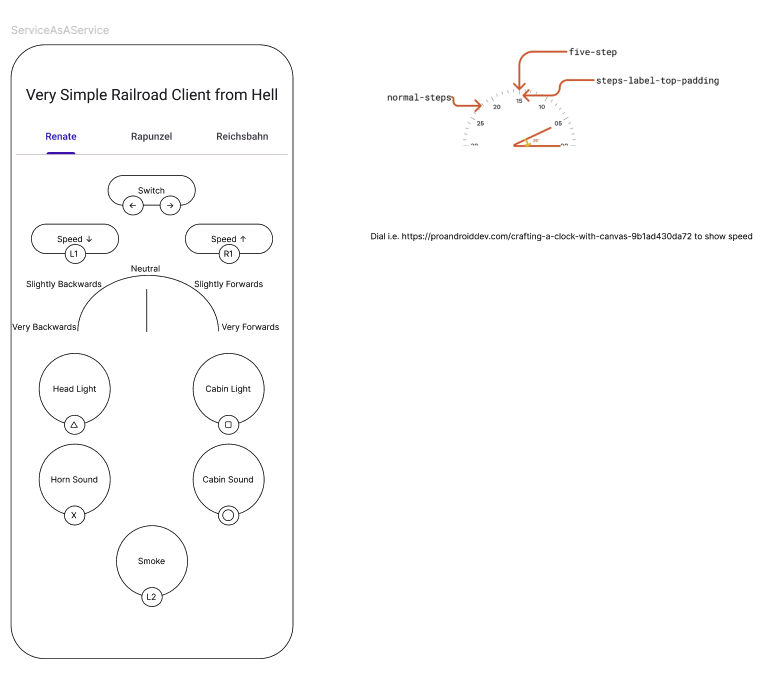
\includegraphics[width=14cm]{images/mockup.png}
        \end{bafigure}
        \begin{bafigure}[
                source={Eigene Darstellung},
                label={fig:ZD1}
            ]{Zustandsdiagramm AttributeCard}
                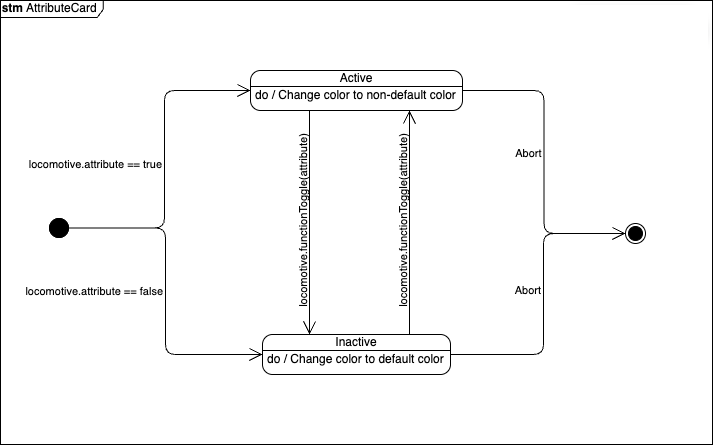
\includegraphics[width=14cm]{images/AttributeCard.png}
        \end{bafigure}
        \begin{bafigure}[
                source={Eigene Darstellung},
                label={fig:ZD2}
            ]{Zustandsdiagramm ButtonPressedIndicator}
                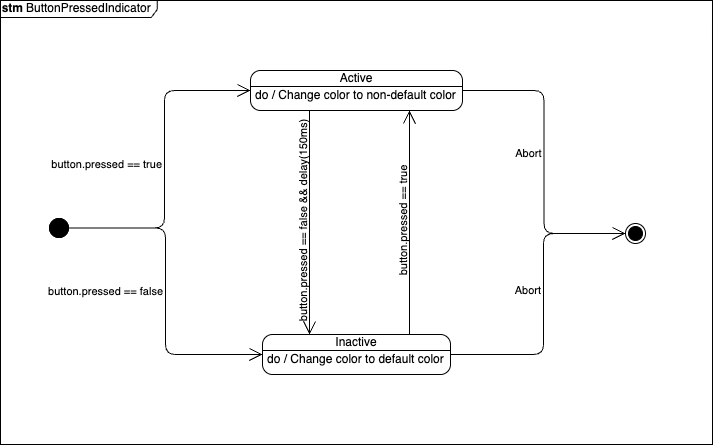
\includegraphics[width=14cm]{images/ButtonPressedIndicator.png}
        \end{bafigure}
        \begin{bafigure}[
                source={Eigene Darstellung},
                label={fig:ZD3}
            ]{Zustandsdiagramm SpeedDial}
                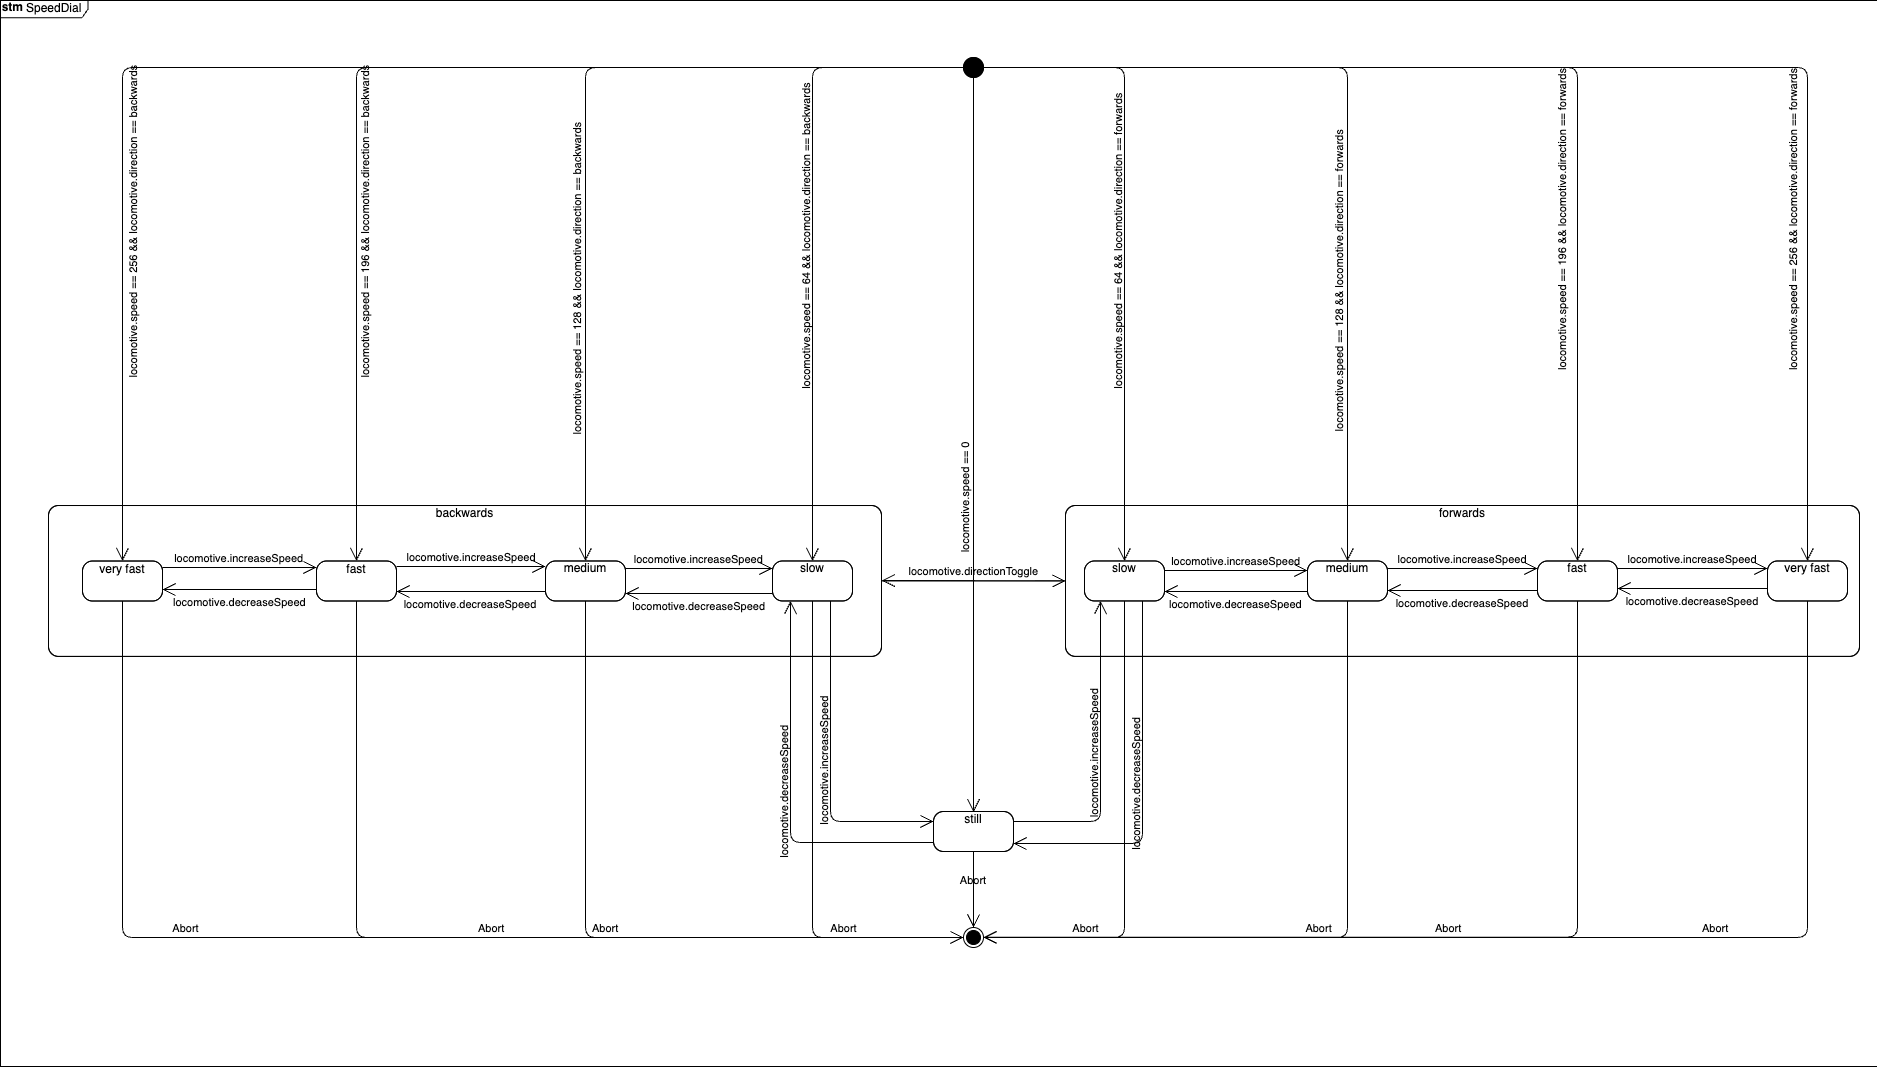
\includegraphics[width=14cm]{images/SpeedDial.png}
        \end{bafigure}

        Die für die Implementierung relevanten Dateien sind HardwareController.kt, LocomotiveController.kt, RailroadViewModel.kt, NewChips.kt, SpeedDial.kt und LocomotiveScreen.kt. \\
        In LocomotiveController.kt definiert die Klasse ControllerInput die Funktionen, die durch eine Controllereingabe ausgeführt werden können. 
        Eine Klasse FunctionType wurde hinzugefügt, um zwischen den verschiedenen Attributen einer Lokomotive zu unterscheiden, die ein-/ausgeschaltet werden können. \\
        In HardwareController.kt werden in der Klasse HardwareController die verschiedenen KeyEvents, die erzeugt werden, wenn ein Knopf oder eine Taste gedrückt wird, den verschiedenen Funktionen zugeordnet.
        Hier erfolgte eine Erweiterung um eine Funktion processMotionEvent, um die Eingabe von non-binären Schultertasten zu ermöglichen. \\
        In RailroadViewModel.kt wurde in der Klasse RailroadViewModel wurde die Datenklasse ControllerHighlightState, die die booleanschen Zustände der hervorgehobenen Benutzeroberflächenelemente als Attribute enthält, definiert und als MutableStateFlow instanziiert.
        Der MutableStateFlow erlaubt das Teilen der im Flow enthaltenen Daten zwischen mehreren Objekten und der Aktualisierung der Objekte nach einer Änderung der Daten.
        Zudem wurde eine Funktion pulseHighlight hinzugefügt, die den MutableStateFlow mit neuen Daten aktualisiert, 150 Millisekunden wartet und dann den MutableStateFlow zurücksetzt.
        Durch die Attribute im MutableFlow werden die Elemente der Benutzeroberfläche konditionell gefärbt.
        In der Funktion handleControllerInput wurde für jede in ControllerInput definierte Funktion die Funktion pulseHighlight hinzugefügt, wobei für jede definierte Funktion das korrespondierende Attribut im MutableStateFlow auf true geändert wird. \\
        Die tatsächliche Benutzeroberfläche beschränkt sich auf die Dateien LocomotiveScreen.kt, NewChips.kt und SpeedDial.kt.
        In NewChips.kt werden die Benutzeroberflächenelemente definiert, die die Funktionen des Controllers, die Tastenbelegung und teilweise den Zustand der Attribute der Lokomotive anzeigen.
        Für die Darstellung der Geschwindigkeit und Richtung wurde aus kreativen Zwecken ein Tachometer gewählt, das in SpeedDial.kt definiert ist
        LocomotiveScreen.kt enthielt die originale Benutzeroberfläche für die Steuerung der Lokomotiven.
        Die neuen Elemente aus SpeedDial.kt und NewChips.kt werden in LocomotiveContent zu einer kohärenten Benutzeroberfläche zusammengestellt. 
        Zudem werden die Elemente mit dem MutableStateFlow und dem geladenen Lokomotivenobjekt verbunden.
        Die finale Version der Benutzeroberfläche ist in den Abbildungen \ref{fig:newUIbase}, \ref{fig:newUIb} und \ref{fig:newUIa} dargestellt. 
        
        \begin{bafigure}[
                source={Eigene Darstellung},
                label={fig:newUIbase}
            ]{Die entstandene Benutzeroberfläche}
                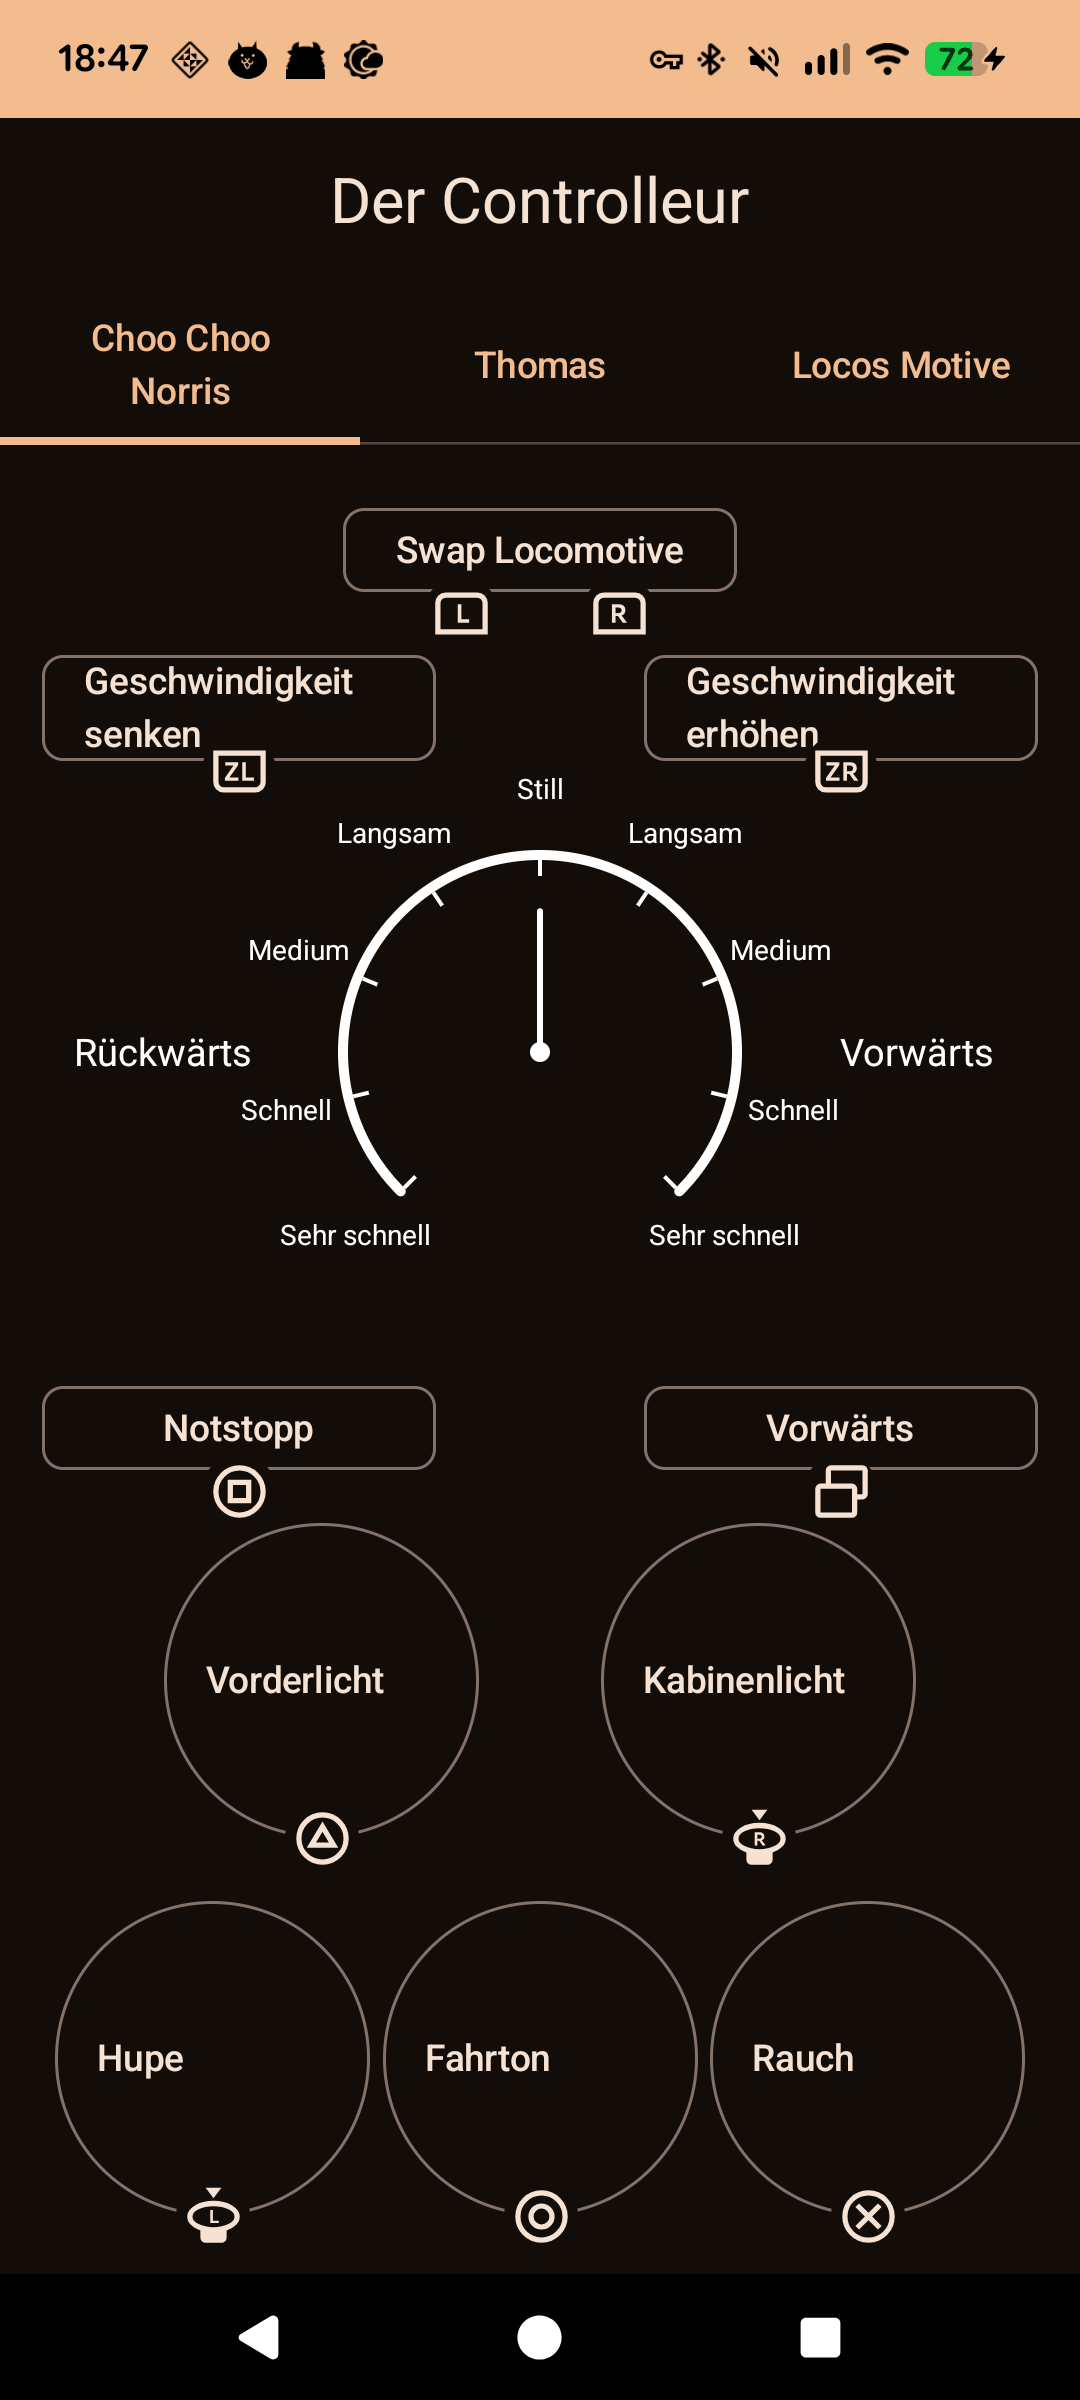
\includegraphics[width=4cm]{images/UIdefaultnew.png}
        \end{bafigure}
        \begin{bafigure}[
                source={Eigene Darstellung},
                label={fig:newUIb}
            ]{Die Benutzeroberfläche ändert sich durch das Drücken eines Knopfes}
                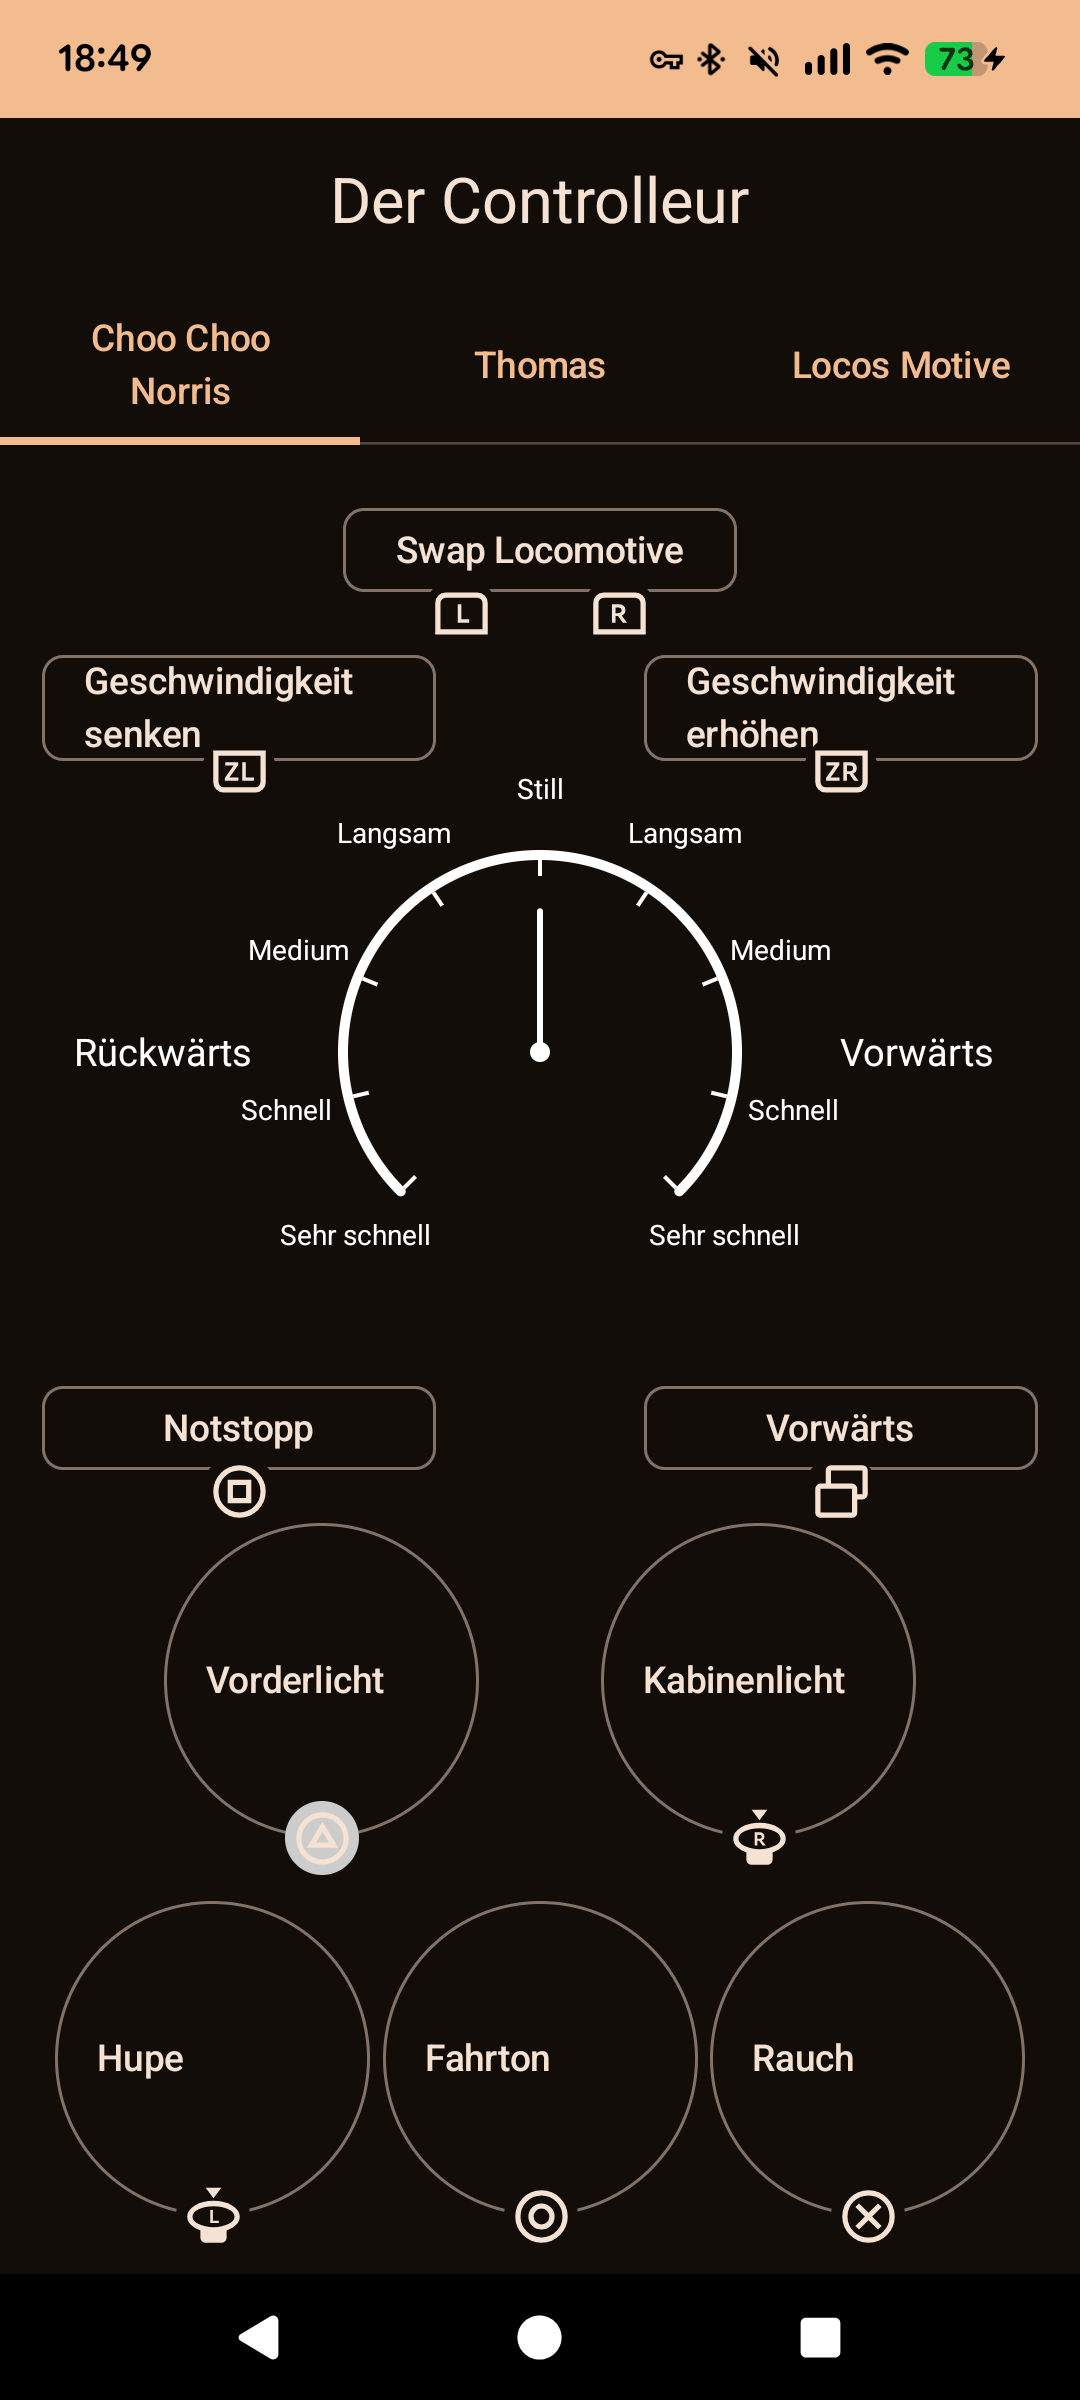
\includegraphics[width=4cm]{images/UIbuttonpressed.png}
        \end{bafigure}
        \begin{bafigure}[
                source={Eigene Darstellung},
                label={fig:newUIa}
            ]{Die Benutzeroberfläche ändert sich, weil die Geschwindigkeit der Lokomotive geändert und ein Attribut der Lokomotive auf true gesetzt wurde}
                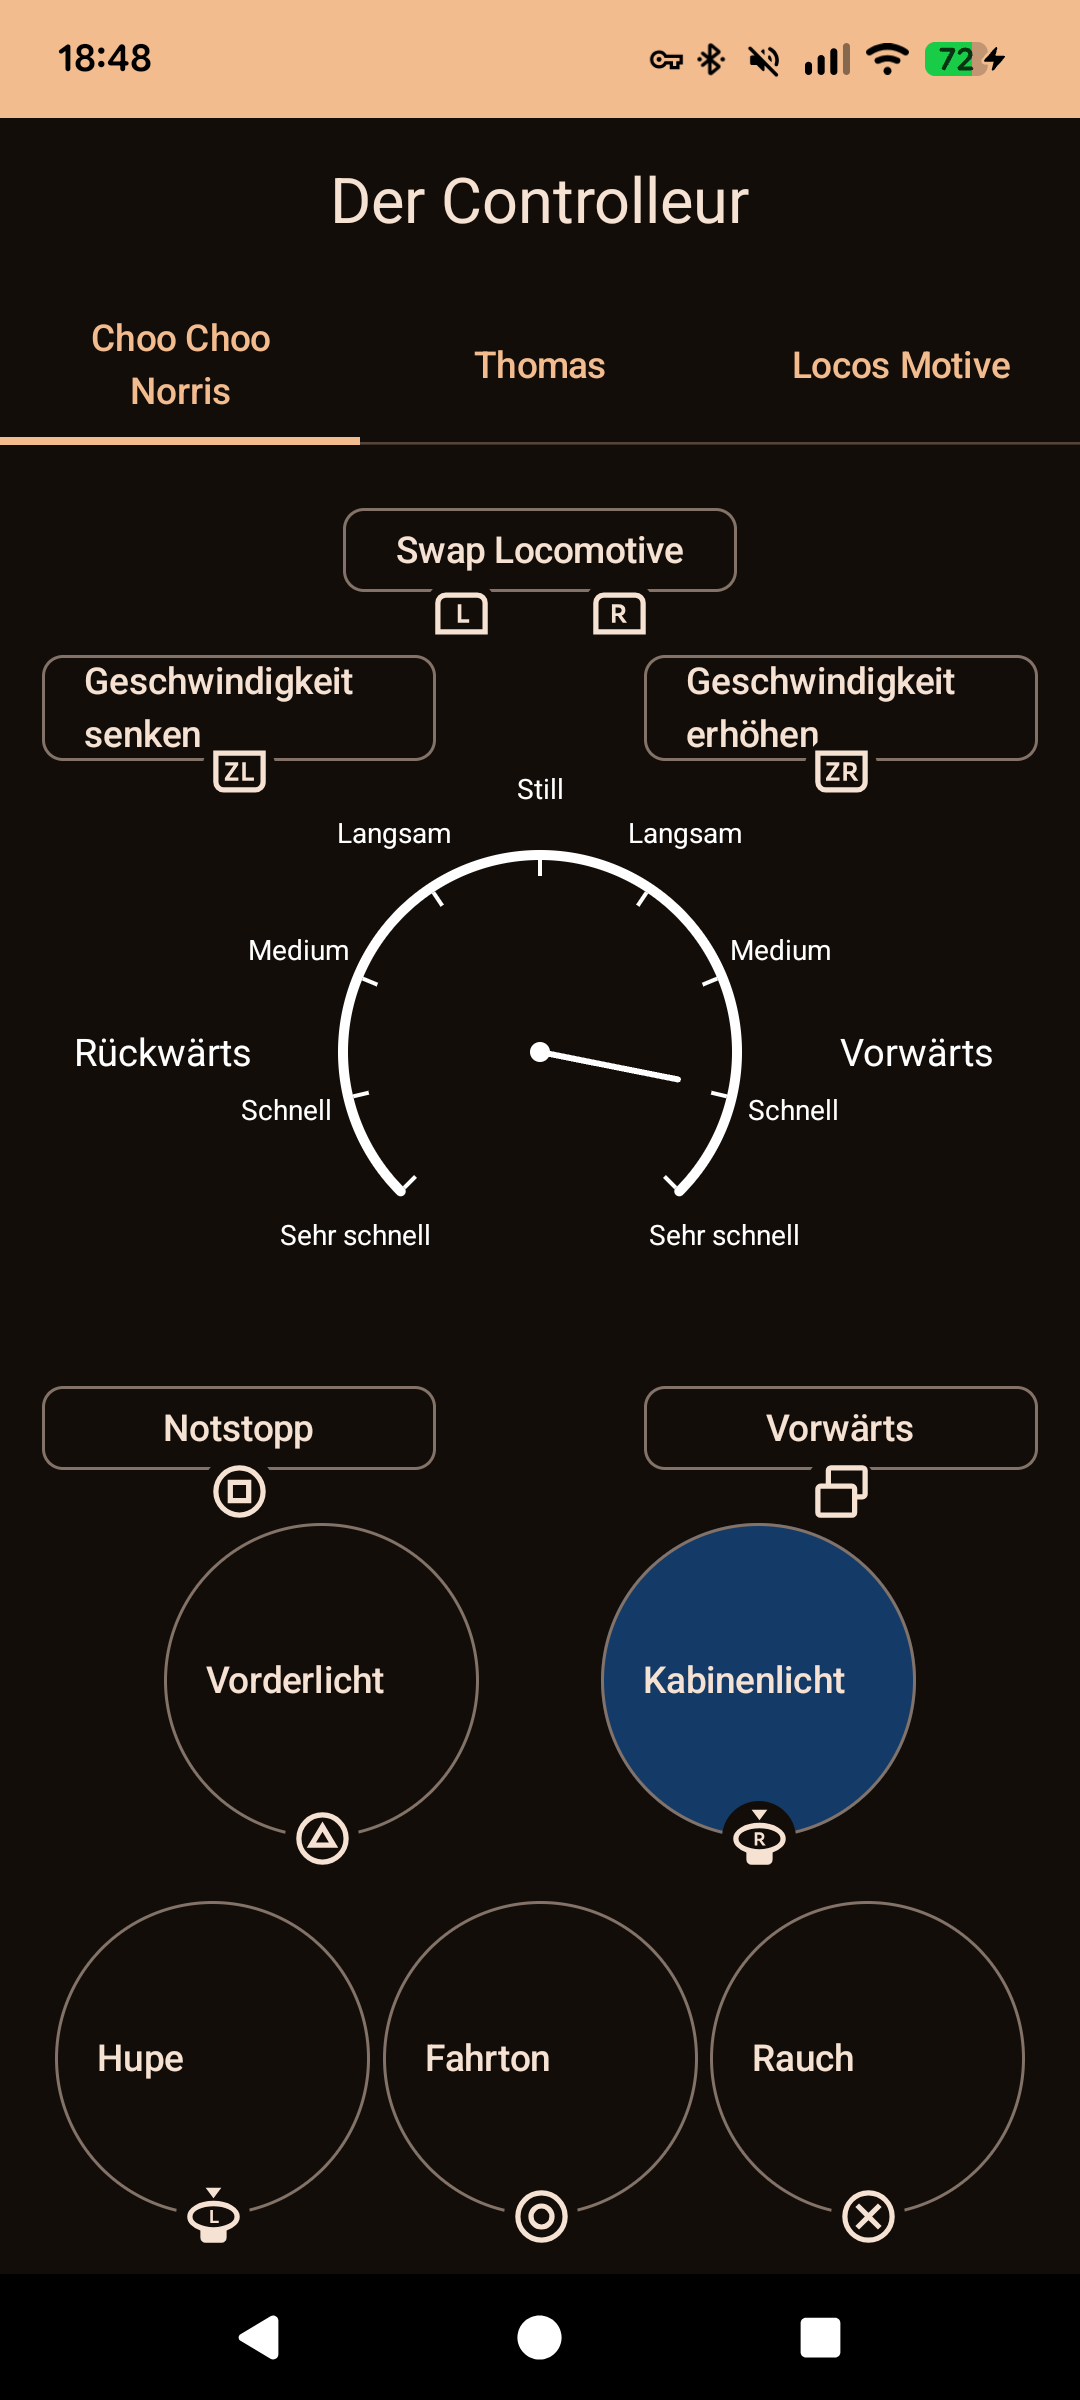
\includegraphics[width=4cm]{images/UIattributechanged.png}
        \end{bafigure}
    \newpage
    \section{Analyse} \label{sec:anal}
    In diesem Abschnitt sollen die in Kapitel \ref{sec:intro} formulierten Analyseziele durch die Beantwortung von Fragen erreicht werden.

    Wie wurden Zustandsdiagramme verwendet?
    
    In Anbetracht der von Rumpe genannten Anwendungszwecke (vgl. Abbildung \ref{fig:usecases}) können die Zustandsdiagramme in die Darstellung des Lebenszyklus bzw. Implementierungsbeschreibung des Verhaltens eines Objekts eingeordnet werden. 
    Die Objekte sind in diesem Fall Elemente der Benutzeroberfläche.
    Das Diagramm ButtonPressedIndicator modelliert die unten an den Chips sich befindenden Icons, die bei Drücken des korrespondierenden Knopfes die Farbe ändern, das Diagramm AttributeCard modelliert die Chips, die ein Attribut der Lokomotive wiederspiegeln, und das Diagramm SpeedDial modelliert das Tachometer.
    Die verschiedenen Anzeigeformen der Elemente der Benutzeroberfläche, die aufgrund von Änderungen in den zugrundeliegenden Daten entstehen, werden als Zustände aufgefasst.
    Die Schaltbedingungen werden teilweise als Methode eines Objekts, teilweise als Boolean dargestellt. 
    Das kann daran liegen, dass manche Methodenaufrufe als Trigger für eine Zustandsänderung dienen, dass im Code die Zustände teilweise auch als konditionelle oder booleansche Variablen dargestellt werden und eine Änderung der Kondition eine Änderung des Zustands darstellt.
    Die Zustandsdiagramme wurden verwendet, um die Zustandslandschaft der einzelnen Benutzeroberflächenelemente zu modellieren.
    Zusätzlich konnten relevante Variablen und Methoden identifiziert und modelliert werden, die die Zustandsänderung hervorrufen.
    Unter der Prämisse, dass nur Menschen einen Knopf betätigen sollen, kann das Diagramm ButtonPressedIndicator auch als Modell einer Interaktion, spezifisch der Mensch-Maschine-Interaktion, interpretiert werden.
    Dies widerspricht jedoch der Prämisse aus Rumpe\vglcite[149]{Rumpe2011}, dass Zustandsdiagramme nur für die Verhaltensmodellierung und nicht für die Modellierung von Interaktionen genutzt werden sollen.

    Sind die Zustandsdiagramme korrekt?
    
    Die Diagramme sind syntaktisch korrekt.
    Es wurden folgende semantische Unklarheiten bzw. Fehler gefunden gefunden:
    \begin{enumerate}
        \item Die Notation für Transitionen ist [<trigger> [',' <trigger>]*['['<guard>']']['/'<behavior-expression>]].\vglcite[331]{OMG2017}
        Einen Trigger als einen Boolean zu notieren ist syntaktisch nicht falsch, kann aber zu Verwirrung führen, da Booleans meistens für guard-Bedingungen verwendet werden.
        \item Im Diagramm SpeedDial existieren zwei Transitionen zwischen den Zuständen \enquote{backwards} und \enquote{forwards}. 
        Da die Zustände Subzustände enthalten, jedoch keinen Pseudo-Startzustand, ist kein sog. Default Entry Behavior definiert. 
        Daraus folgt, dass der Zustandsautomat nach der Transition terminiert oder das das Diagramm formal ungültig ist.\vglcite[309f]{OMG2017} 
    \end{enumerate}
    
    Konnte der Verwendungszweck erfüllt werden?

    Angesichts der im vorherigen Paragraph benannten Fehler wäre eine Verneinung der Frage durchaus berechtigt. 
    Es ist jedoch zu bemerken, dass neben einer Sicht des Modells auf das modellierte Objekt ebenfalls die Sicht des Betrachters auf das Modell existiert, was eine subjektive Sichtweise auf ein Modell bedingt.
    Dies ermöglicht die Bildung eines semantisch kohärenten Modells innerhalb der subjektiven Sichtweise entgegen des semantisch inkorrekten Modells, insbesondere wenn der Betrachter sich nicht den unterliegenden Formalismen zur Betrachtung des Modells bekannt ist.
    In Anbetracht dessen, dass die Benutzeroberfläche von genau einer Person implementiert wurde, kann der Verwendungszweck, das Modell als Vereinfachung eines Gegenstands zur Erleichterung der Untersuchung zu nutzen, durchaus erfüllt werden.
    Ob andere geplante Verwendungszwecke erfüllt werden konnten, kann an dieser Stelle nicht geprüft werden.

    \newpage
    \section{Verifizierung und Validierung} \label{sec:vnv}
        \subsection{Verifizierung als wissenschaftliches Schreibprojekt}
        Die Verifizierung dieser Arbeit als wissenschaftliche Arbeit orientiert sich an Abschnitt 1.3 \enquote{Allgemeine Anforderungen an wissenschaftliche Schreibprojekte} des Leitfaden für wissenschaftliche Arbeiten (verk.) \bacite{Grassmann2017}. Es werden relevante Anforderungen als Zitate aus der Quelle übernommen und geprüft.

        \enquote{Dafür verfügen Sie über die notwendigen Fachkenntnisse. Genaugenommen ist deren Erarbeitung also nicht Teil Ihrer Schreibprojekte.}

        Die Fachkenntnisse, die für die Erstellung dieser Arbeit notwendig waren, waren vor der Erstellung nicht ausreichend vorhanden.
        Dies ist bedingt durch die Themenauswahl, die durch den von dem Dozenten gesetzten Rahmen ermöglicht wurde, eine spezielle Teilmenge der eigentlichen Themen darstellt (UML - Zustandsdiagramme, Benutzeroberflächen - Benutzeroberflächenentwicklung) und zusätzliche Literaturrecherche benötigte.
        Nach der Bearbeitung wurden die notwendigen Fachkenntnisse akquiriert.

        \enquote{Um Ihren Eigenbeitrag tatsächlich beurteilen zu können, ist es wichtig, dass Sie sorgfältig kennzeichnen, welche Inhalte Sie von anderen übernommen haben}

        Die Zitierung wird den formalen Vorgaben gerecht vorgenommen.
        Eine Dokumentation der KI-Nutzung wird in einem zusätzlichen Dokument vorgenommen.
        Die Gliederung dieser Arbeit wurde von Michael L. inspiriert. {LM}
        Sonstige Hilfe wurde nicht bezogen.

        \enquote{Darüber hinaus haben Sie Ihre Arbeiten immer auf der Grundlage anerkannter wissenschaftlicher Prinzipien Ihrer jeweiligen Disziplin anzufertigen.}

        Relevante Prinzipien (Erkenntnisorientierung, Nachvollziehbarkeit, Empirische Fundierung, Theoriebezug, ...) wurden beachtet.

        \enquote{[...] Verwendung von anerkannten [, aufgabengerechten] Methoden Ihres Fachgebietes bzw. Ihrer Disziplin.}

        Die Fallstudie ist eine in der Wirtschaftsinformatik anerkannte Methode.

        \enquote{Zudem wird von Ihnen erwartet, dass Sie systematisch an die Bearbeitung resp. Lösung Ihrer jeweiligen Aufgaben- bzw. Problemstellung herangehen.}

        Das System für die Lösung der Aufgabe war durch die Struktur der Lehrveranstaltung sowie der Methodik vorgegeben.

        Insgesamt ist eine Nichterfüllung der ersten Anforderung zu verzeichnen. Damit ist diese Arbeit kein wissenschaftliches Schreibprojekt.

        \subsection{Validierung}
            \subsubsection{Wissenschaftliche Relevanz}    
            Disterer definiert wissenschaftliche Aussagen als relevant, wenn sie \enquote{Fragen von Interesse beantworten}.\vglcite[23]{Disterer2014} Die wissenschaftliche Aussage dieser Arbeit beantwortet die Forschungsfrage \enquote{Wie können \gls{UML}-Zustandsdiagramme in der Entwicklung von Benutzeroberflächen genutzt werden?}.
            Das Interesse des Autors an der Frage ist durch die Aufforderung des Dozenten, Interesse an den bearbeiteten Themen und der Beantwortung der Frage zu haben, begründet. 
            Für die breitere wissenschaftliche Gemeinschaft könnte die Frage von Interesse sein, da deklarative Oberflächen in der Benutzeroberlächenentwicklung starkes Wachstum verzeichnen. 
            In der Webentwicklung sind Web-Technologien wie React, Next.js,Vue.js oder Svelte sowohl bei angehenden als auch bei professionellen Entwicklern sehr beliebt.\vglcite{stackoverflow}
            Die Bedeutung von Zustandsdiagrammen für zustandsbasierte Benutzeroberflächen konnte nicht vollständig geklärt werden.
            Diese Arbeit soll jedoch einen Ansatz für die Verwendung geben.

            Die wissenschaftliche Aussage dieser Arbeit ist in ihrer Aussagekraft beschränkt. 
            In der vorliegenden Fallstudie wurden nur Dokumente und Artefakte als Analyseobjekte betrachtet
            Zudem wurde lediglich ein Fall betrachtet,der zudem kaum Bezug auf die tatsächliche Praxis der Benutzeroberflächenentwicklun aufgrund von unter anderem der Teamgröße hat.
            Die Konzeption als deskriptive Fallstudie bedingt zudem einen geringeren Erkenntniswert als eine vergleichbare explorative oder explanative Fallstudie.\vglcite{Riedel2006}

            \subsubsection{Relevanz der Arbeit für den Autor}
            Diese Arbeit stellt für den Autoren die dritte (wissenschaftliche) Schreibarbeit an der Dualen Hochschule Sachsen in Dresden dar. 
            Der Nutzen der Akquise der Fallstudie als wirtschaftswissenschaftliche Methodik ist voraussichtlich hoch, da sie in zukünftigen Arbeiten ebenfalls verwendet werden kann.
            Zudem ist ein hoher Wissenszuwachs in den Gebieten UML, Beschreibung von Standards, Finite Automatentheorie, Modellierung mit Zustandsdiagrammen, Validierung und Verifizierung von Ergebnissen sowie der Gartenbahn zu verzeichnen.


    \newpage
    \section{Fazit und Ausblick}
    In dieser Arbeit sollte die Forschungsfrage \enquote{Wie können \gls{UML}-Zustandsdiagramme in der Entwicklung von Benutzeroberflächen genutzt werden?} beantwortet werden. 
    Dazu wurden in Kapitel \ref{sec:theory} die Grundlagen zu \gls{UML}-Zustandsdiagrammen und der Entwicklung von Benutzeroberflächen.
    Für die Beantwortung der Frage wurde in Kapitel \ref{sec:meth} die Fallstudie als Methodik gewählt.
    Der relevante Fall wurde in Kapitel \ref{sec:case} beschrieben und Dokumente und Artefakte wurden in Kapitel \ref{sec:anal} analysiert.
    Anschließend wurde ein Verifizierung dieser Arbeit auf den Status als wissenschaftliche Schreibarbeit und eine Validierung der Relevanz in Kapitel \ref{sec:vnv} durchgeführt.

    In der Theoriebetrachtung wurden bereits andere Arbeiten identifiziert, die Zustandsdiagramme für die Entwicklung von Benutzeroberflächen genutzt haben. 
    Es wurde identifiziert, dass Zustandsdiagramme zur Modellierung von Funktionen, und in Form von SCXML in der Entwicklung und Zustandsmodellierung von 3D-Oberflächen sowie der Implementierung durch XState genutzt werden können. 
    %hier beschreiben, wie sie benutzt wurden

    Anhand des beschriebenen Falls konnte ein weiterer potentieller Anwendungsfall identifiziert werden. \gls{UML}-Zustandsdiagramme können in der Benutzeroberflächenentwicklung zur Modellierung der Zustandslandschaften von Elementen der Benutzeroberfläche genutzt werden. Zusätzlich können mit Hilfe der \gls{UML}-Zustandsdiagramme für Zustandsänderungen relevante Variablen und Methoden identifiziert werden.

    In zukünftigen Fallstudien kann der Rahmen der Fallstudie durch eine vergleichende oder explanative oder explorative Fallstudie erweitert werden. 
    Zudem können praxisnährere Fälle aus beispielsweise Unternehmens- oder Open-Source-Kontexten genutzt werden, um unter anderem die Anwendbarkeit bei größeren Entwicklerteams zu bestimmen.

    \newpage
\end{basimple}
\end{document}
